\subsection{Hybrid Merkle Tree}
A hybrid Merkle tree is a data structure that combines the benefits of both sparse Merkle trees (SMT) and quad Merkle trees. It achieves this by having three child nodes instead of the traditional two or four child nodes.

\begin{figure}[H]
    \centering
    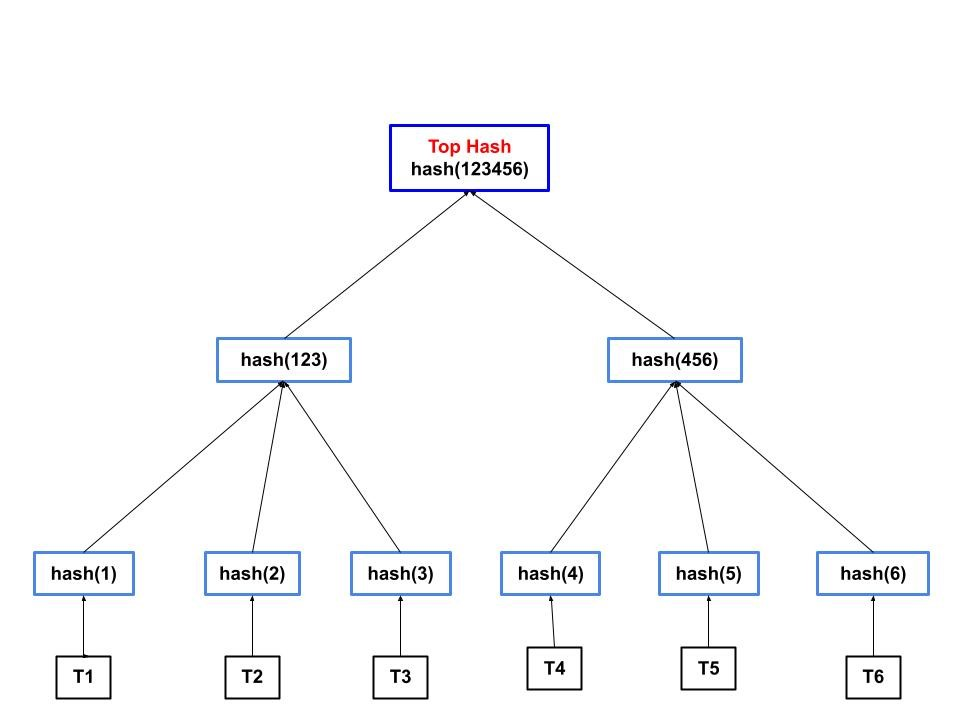
\includegraphics[scale=0.6]{figures/Hybrid Merkle Tree.jpg}
    \caption{Hybrid Merkle Tree}
 
\end{figure}